\section{B9 \& Beyond! - Planika Jama}

\begin{marginfigure}
      \checkoddpage \ifoddpage \forcerectofloat \else \forceversofloat \fi
      \centering
              \frame{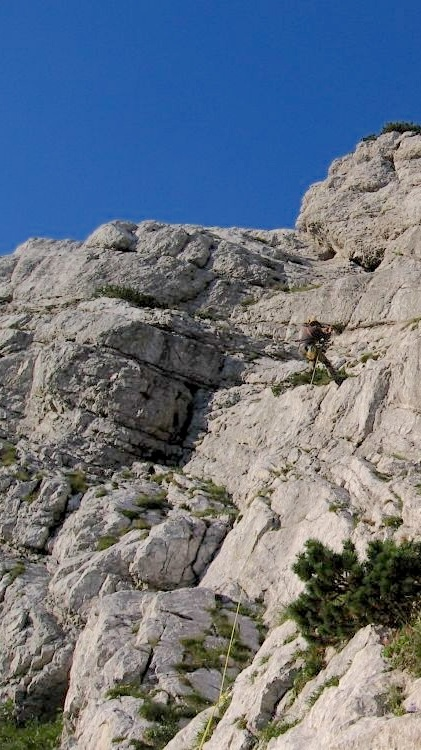
\includegraphics[width=\linewidth]{2007/b9/jana carga - planika - cliff abseil--orig.jpg}} 
  \caption{The \passage{Planika} cliff abseil. \pic{Jana Čarga}}
\end{marginfigure}

\margininbox{B9}{
     \begin{itemize}
    \item Aljošha Bončina
    \item Špela Leban
    \end{itemize}}{\explo}

Walking briefly over to \passage{B9} the day after the super-action, we could spot
the cairn I left down near \passage{Primadona}. Combined with one placed by
Jana \& I on the headland near \passage{U-Bend}, suddenly the whole complicated 3D
structure fell into place. Neither of the caves we could see from near
B9 were \passage{Primadona}, though the entrances looked similar - both
were new caves in an area never visited!

The next day we were joined on the plateau by some of the young JSPDT.
Jana \& I went with Alijosha and Spela to \passage{B9}, and explained the
situation. The weather was awful - thick cloud everywhere. While the
Slovs re-explored bits of \passage{B9} and checked to see if anything had changed
after the earthquake\sidenote {occurred 1998 \& 2004} (a pitch had disappeared off the original survey as
a bit of the cave collapsed and turned into a boulder climb!), I placed
two bolts for the descent down the cliff. This was really quite
exhilarating - a gale swept over the edge of the plateau, the rock was
soaked and slippery, and every now and then the thick clouds would part
for a glimpse of \passage[mountain]{Krn} or the \passage[river]{Tolminka} valley a very long way away!

The next day Aliosja and Spela went down from the plateau, so Jana and I
went back alone to \passage{B9} to rig down the cliff. The weather was much
improved! Jana abseiled down first and went investigating the three cave
entrances, while I came down behind and put in the rebelay bolts. The
three entrances were very interesting - the main one contained an
enormous aven which connected back up to the headland above \passage{U-Bend} (you
could see the sky through the top), but was an enormously steep boulder
slope with useless rock. The further entrance was a crawl in boulders
that was only briefly pushed by Jana. The smallest, highest entrance was
the most immediately interesting - a perfect metre by metre triangular
arch which led directly to a deep pitch. 

A shimmer of white was just
visible at the bottom. Bolts were placed for a traverse along a
beautiful slab of limestone to save freeclimb on the steep bowl valley
edged with a cliff, and the main hang bolt + first rebelay was placed
for the small-cave pitch, finishing our 100 m rope. We decided to name
this new cave \passage{Planika} Jama, after the rare mountain flower that covers
the sun-kissed (\& adder infested!) slopes around \passage{B9}.

\begin{marginfigure}
      \checkoddpage \ifoddpage \forcerectofloat \else \forceversofloat \fi
      \centering
              \frame{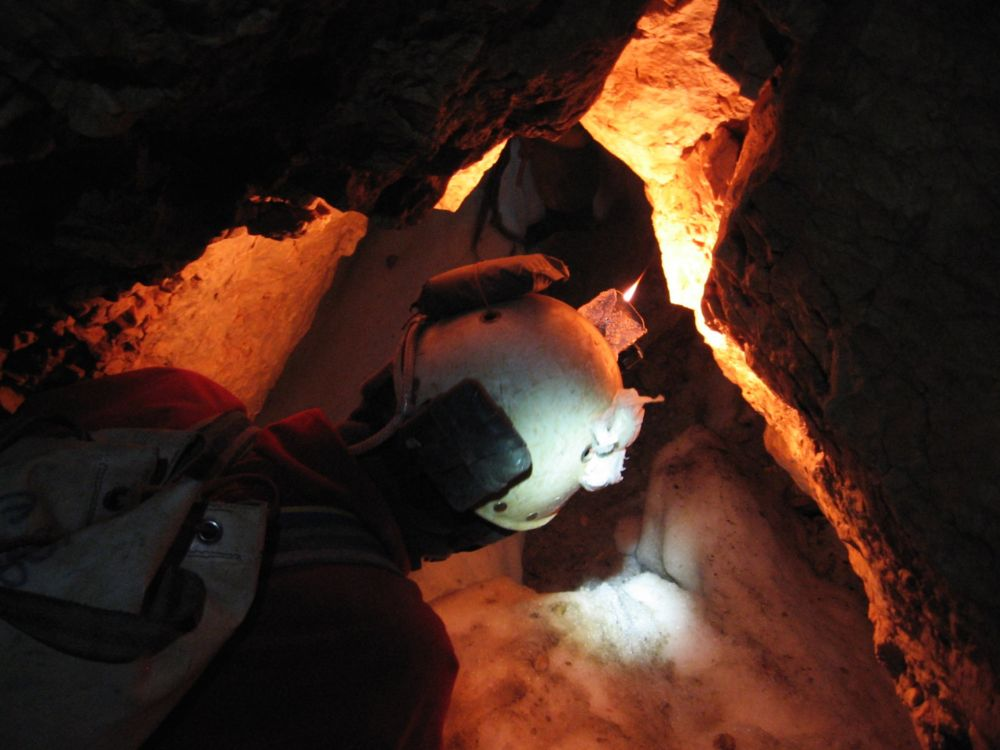
\includegraphics[width=\linewidth]{2007/b9/jarvist frost - planika - rock arch--orig.jpg}} 
  \caption{The triangular rock arch in \passage{Planika}. \pic{Jarvist Frost}}
\end{marginfigure}

Rather confusingly, we could occasionally hear echo-y shouts bouncing
around from below as we walked about the bowl valley, inevitably
disturbing stones. We tried to be as careful as we could, but couldn't
really understand what was going on - except for the fact that one of
the voices sounded like Kos.

Once back on the plateau, Jana pieced together the situation by mobile -
Alijosha and Spela had gone down to \passage{Kal}, taken the ICCC rigging gear
left in the third hut and went to the lower cave entrance pointed out to
them the day before via an abseil down the cliff near \passage{Primadona}
where I had placed the cairn on the Ping Pong Ball Bombe action. Jana
went down to \passage{Kal} to discuss the situation that evening and came back up
the next day rather upset. The new cave was to be called \passage{Monatip}
(`Fucking Idiot' in the local dialect).

\margininbox{Planika Jama}{
 \begin{itemize}
\item Jana Čarga
\item Jarvist Frost
\end{itemize}}{\explo}

\begin{marginfigure}
\centering 
  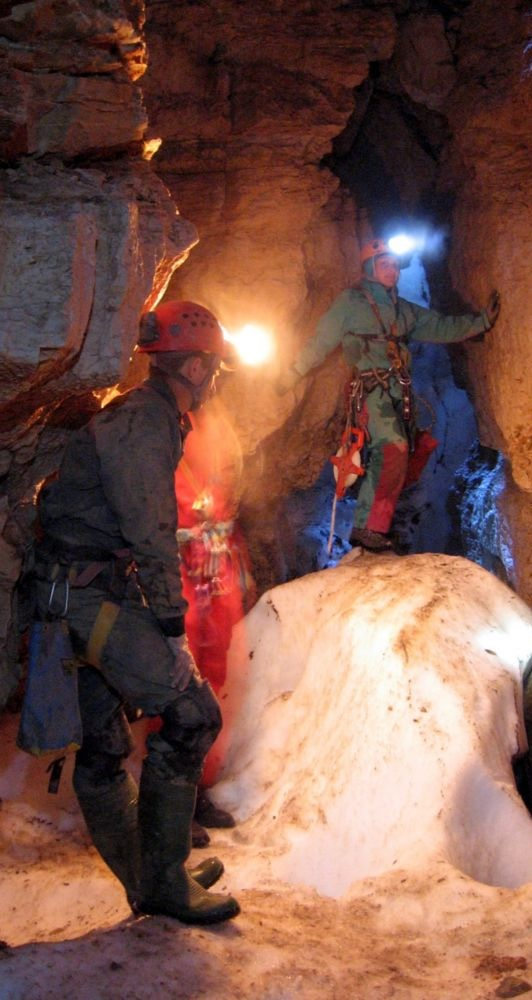
\includegraphics[width=\linewidth]{2007/b9/jarvist frost - planika - acre lane--orig.jpg}
  \caption{\passage{Acre Lane} in \passage{Planika Jama}. \pic{Jarvist Frost}}
\end{marginfigure}

The next day started with Goaty \& Jarv surface surveying to \passage{B9}. Jana
and I then descended the clif, surveying as we went. Again, within the
cave, we used the efficient technique of the lightweight Jana abseiling
down past rub-points, followed by Jarv bolting the rebelays behind while
Jana explored the next bit. The pitch was perhaps the most beautiful
entrance pitch on the Mig plateau. From a bolt placed in the ceiling a
hang dropped down past a fridge-sized boulder before swinging out to a
rebelay (placed by using my walking boot heel `skyhook'). 

From here one
abseiled down an almost perfect brick wall, above an enormous snow plug,
before swinging into a little dry streamway cascade to finish the last
bolt to land on the snow plug, which contained a large metre wide 6 m
deep hole bored out of the ice by wind or water, and similar, more
narrow, gaps on the edges of the plug. A small rift led off and
immediately closed down. 

From the top of the snow plug Jana found a
crawl way under a rock bridge to a climb up on ice on one side and rock
on the other (the ice was a more reliable foothold!), to reach a
snow-filled chamber which was daylight flooded and clearly below the
slope of the large entrance. An ice traverse in this chamber (we named
it \passage{Yorkshire Pudding}, as it was a torus of snow with a dimpled center).

From the far side of the Yorkshire pudding one could squeeze down
between the rock and snow, attempt a climb past a stack of wedged
boulders towards the aven, or walk down a snow-bottomed meander. The
meander we named \passage{Acre Lane} after our London home. This meander
suddenly regained a rock floor and led on to a tight rift which seemed
to be a small pitch head. There were a lot of boulders strewn around.
Here we PSS'ed and headed back.

The next day we were joined by Andreja \& James H. Jana and Andreja
bolted the backup bolt for this new traverse, while I gardened my way
along the tight rift and then placed a bolt holding myself in place
within the rift by breathing in until my ribs were wedged securely! This
was perhaps the slowest bolt I've every placed as I was lying sideways
with the arm holding the driver bent back behind my head, and the hammer
cocked under my buoy, while considering the 6 m drop to the floor! It
was with some relief that I took the rope through from the girls and
rebelayed my way down.

\margininbox{Planika Jama}{
     \begin{itemize}
    \item Jana Čarga
    \item Andreja Fratnik 
    \item Jarvist Frost
    \item James Huggett
    \end{itemize}}{\explo}

Around the corner the cave got strange once more - from a rock balcony
one is confronted with a chamber filled with a 45 degree slope of
compacted snow. Exploring around this we found that the upper levels
shut down, but seemed diggable (from the survey it appears that we were
within a metre of the Yorkshire Pud - it must be the same snow slope),
and there was a beautiful inlet which had formed some amazing
ice-pearls. 

The obviously way on was down. The snow steepened and
disappeared down at about 60 degrees with the rock roof not too far
away. Carefully traversing across the snow, I placed a bolt on the wall,
and abseiled down on my back. The ceiling closed in and the rope began
to rub, the walls shut down from both sides. At the bottom I faced the
end of the snow, with a 50cm gap of boulders sitting there.

\begin{marginfigure}
\checkoddpage \ifoddpage \forcerectofloat \else \forceversofloat \fi
\centering
 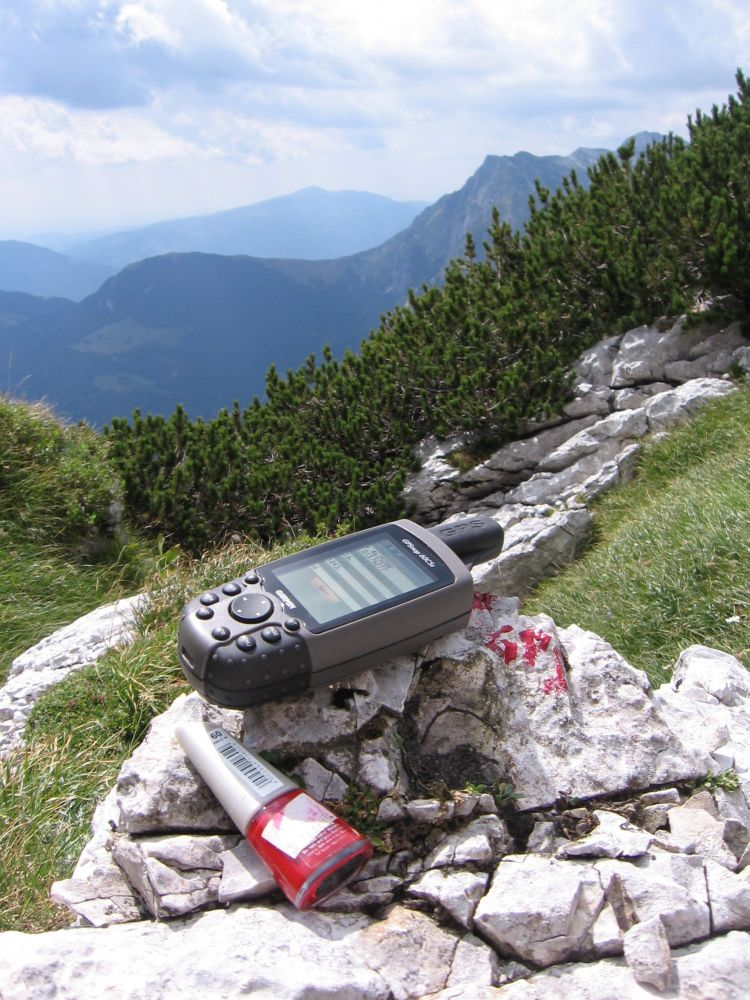
\includegraphics[width=\linewidth]{2007/b9/jarvist frost - b9 boulder cairn gps--orig.jpg} 
 \caption{GPS on the B9 boulder cairn. \pic{Jarvist Frost}}
\end{marginfigure}


The next step was obvious as it was insane - digging at the bottom of a
funnel with a lot of loose rubbish above. By picking up the boulders and
rotating I found I could play tetris, the fitting pieces disappearing
with a gravely rush through the floor. There was a strong draft, what on
earth was I digging towards? With a terrifying series of rock booms and
human shouts almost directly above my head, I pushed myself into the
corner of the snow shoot and hoped for the best. It turned out that the
rift pitch head had been disrupted as someone passed rope through,
collapsing a drystone wall and sending a few hundred kilos of rocks
cascading down. Jana had just reached the rebelay bolt going up,
\bignote{narrowly avoiding being caught in the waterfall of limestone}.

Once I stopped hyperventilating, and accepted that no further boulders
were coming down, I carried on digging with bare (now bloodied hands)
with ten minutes of frantic energy, a way was found. Originally I was
digging alongside the snow, but as it opened up I found I could go
straight down and way. A 5 m climb on boulders took me down to the
strangest chamber I have ever been in. Still attached to the rope, I
stood on a metre wide ledge that ran alongside a wall of perfect white
ice. The ice was wet - drips were everywhere. The ledge continued and
narrowed, snaking alongside this berg. From the middle of the ledge I
saw the strangest sight of my life - a phreatic crawlway winding down at
45 degrees through the ice, distinctly blowing, and with a similar rock
ledge and wall visible on the other side. With no bolt kit and no
camera, I headed out to my shaken compatriots. I was frozen, as my
wellies and cuffs were now packed with snow, and everyone was a little
shaken after the collapse.

  \margininbox{Planika Jama}{
     \begin{itemize}
    \item Ben Banfield
    \item Jana Čarga
    \item Emil Frankič
    \item Jarvist Frost
    \end{itemize}}{\explo}

Our last trip was a speedy survey, photo and derig, with Ben B and Emil.
Jana went down the ice slope but didn't fancy the still unstable boulder
climb, so we surveyed from this edge. The photo-gear was too much of an
effort to get passed the tight rift-pitch. Ben placed his first bolt as
a safety traverse across the ice. After surveying back to above the rift
pitch, we switched to photography documenting the cave as we derigged
out with the rope and metalwork.

Emil and Ben headed back to the Bivi while Jana \& I bolted down with
the Planika rope to reach \passage{Monatip} in order for him \& Izzy to surface
and cave survey the following day. Glorious weather, we sat watching the
sun set behind \passage{Krn}, with the Venetian bay visible beyond.

\name{Jarvist Frost}

\begin{marginfigure}
      \checkoddpage \ifoddpage \forcerectofloat \else \forceversofloat \fi
      \centering
              \frame{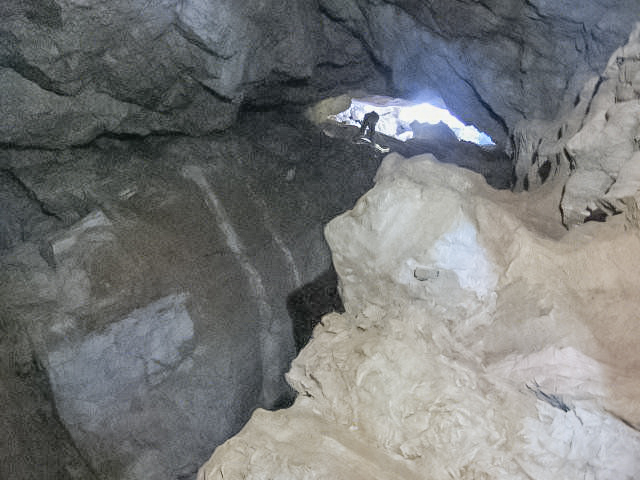
\includegraphics[width=\linewidth]{2007/b9/jarvist frost - planika - entrance pitch1--orig.jpg}} 
  \caption{The \passage{Planika} entrance pitch. \pic{Jarvist Frost}}
\end{marginfigure}

\newpage
\section{Notes on Photography}

\begin{marginfigure}
      \checkoddpage \ifoddpage \forcerectofloat \else \forceversofloat \fi
      \centering
              \frame{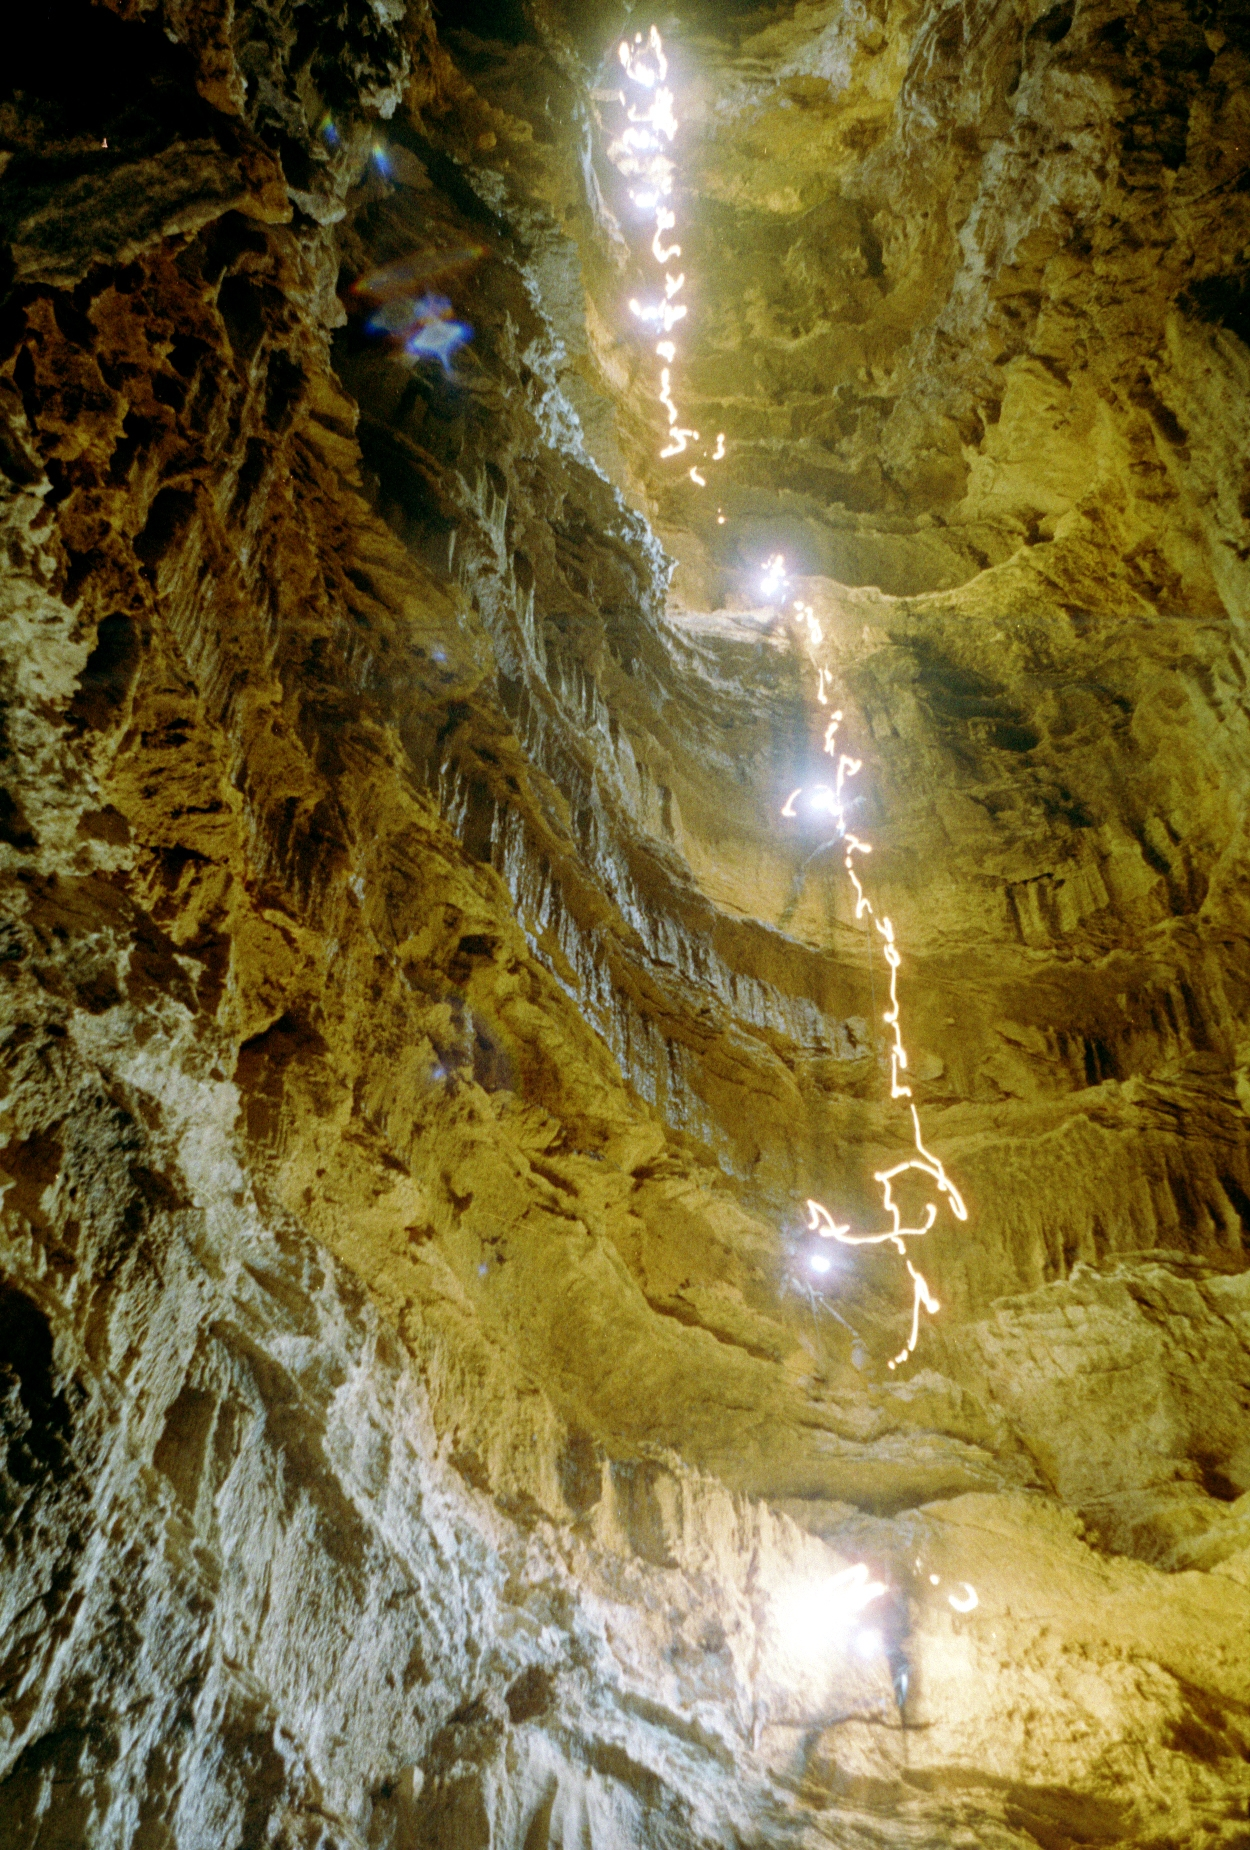
\includegraphics[width=\linewidth]{2007/b9/Clewin_on_Concorde_2004_Photo_by_Jarvist_Frost-highquality--orig.jpg}} 
  \caption{A long exposure shot of Clewin on \protect\passage{Concorde} pitch in \protect\passage{Vrtnarija}, taken in 2004. \pic{Jarvist Frost}}
\end{marginfigure}

\margininbox{That Concorde Photo}{

Zenit EM camera on Bulb (zenit's lock open without needing a seperate remote trigger) with a 49mm Helios lens (standard) at F4. Super cheap 200ASA Bonusprint colour-print film. Flash was fired every \textasciitilde 10 m, mostly at Rebelays and sometimes between. It was, I believe, one Jan's usual flashes, I think with a guide number of around 50. Total exposure was around 15minutes. £13 on eBay Zenit, £2 film, £5 developing - best £20 I've ever spent! \mininame{Jarv}}{\logbook}

\subsection{What Camera?}

Dave Wilson uses fully mechanical Rollei 35s, and has this to say: The 35LEDs take mercury batteries (PX27s?) for metering, which aren't obtainable these days, but there are some fixes available (from the Small Battery Company, I think). I have skylight filters on all the cameras to protect the lenses, and I think I have a couple of ND4s for surface shooting in bright light with fast film (the shutter only goes down to 1/500.

Jarv's cameras:

\begin{itemize}
    \item 35mm Ricoh GR1s/v. Bought from eBay for \textasciitilde£100 smackerones. Small enough to fit in my Peli 1030, and with a built-in timed exposure mode \& both infinite focus \& hyperfocal overrides, crystal perfect 28mm lens. Whoah. Took up mountain in lieu of SLR (Mig 2007) and was much impressed by quality of prints, less impressed by quality of digitisation from film.
    \item Zenit-E. Helios 49mm lens (see Concorde shot), and cheap 28mm F3.5 lens. So manual it hurts. Would probably survive nuclear war. Was quite possibly designed so.
    \item Canon AE-1, with 50mm SSC F1.4 lens and 28mm F3.5 lens. Have two bodies. Unfortunately design is one where the shutter is held open by battery power - so not so good for super super long exposure.
\end{itemize}

The spot-beam of miglights is strong enough to appear in photos as a rather sickly green spot; omni isn't generally strong enough. 


\subsection{Dealing with Noise}
Do you love noise? My Little A520 spews noise across the print. Best results involve the following GIMP flowchart:

    \begin{itemize}
        \item Speckle Reduction
        \item Gaussian blur with Pixel=1.6 (or more, if shot out of focus \& so not worsened by blurring)
        \item Unsharp mask with Pix\textasciitilde1.2 . Amount tuned for effect.
    \end{itemize}

Also: GREYCstoration is a FREE digital camera noise removal program, which both integrates into the GIMP \& as a stand alone utility. It's very very tunable.


\name{Jarvist Frost}
